
\section{Additional Details}
\label{sec-appendix}
\subsection{Activation profile setup}

We forward 1030 LIMA~\cite{zhou2023lima} prompts in order and capture last-prompt-token activations at every transformer-layer output, default generation parameters, no hyperparameter search.
Batch size 4, activations stored in bfloat16.

\subsection{Layer matching}

MSE-guided matching overwhelmingly assigns donor layers to the earliest possible recipient layers (Figure~\ref{fig:llama-mse}).
That disagrees with evidence that semantic functions concentrate in late layers~\cite{tenney2019b} and does not transfer well.
Linear depth matching is the default in the main experiments.

\begin{figure}[htbp]
\centering
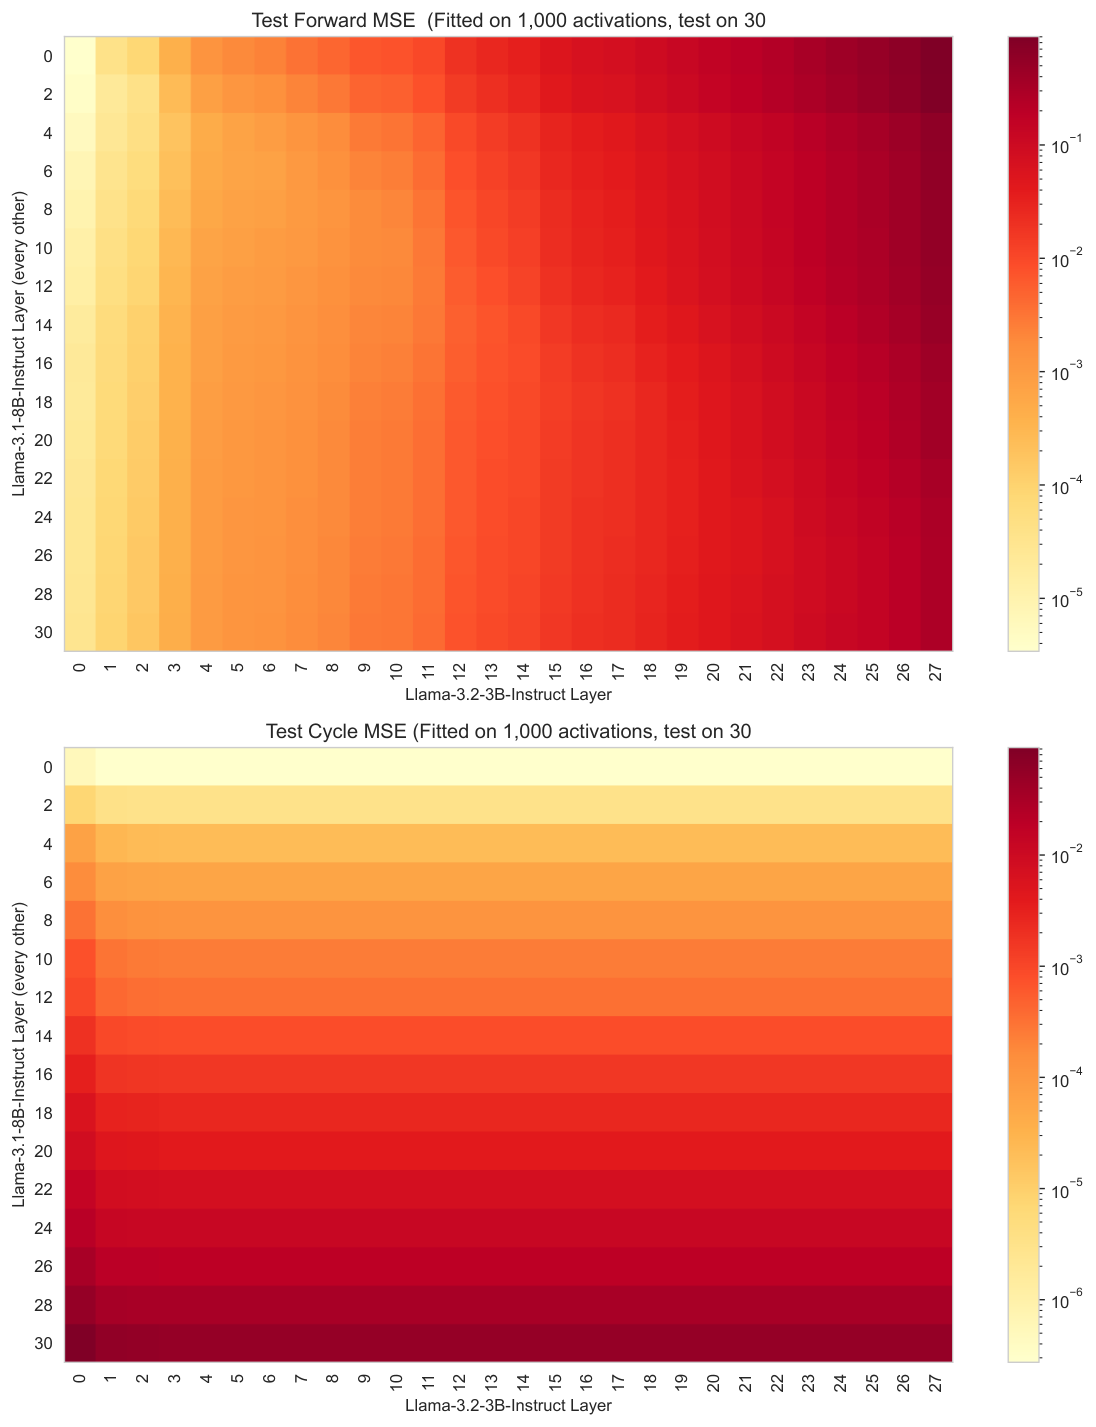
\includegraphics[width=0.8\linewidth]{figures/llama_detailed_analysis.png}
\caption{Llama-3.1-8B-Instruct to Llama-3.2-3B-Instruct test loss, averaged across input.
Minimizing forward or cycle loss is a poor layer-mapping strategy because later layers are harder to reconstruct.}
\label{fig:llama-mse}
\end{figure}

\subsection{Models}

All instruct checkpoints from Hugging Face as of March 2025.

\begin{table}[h]
\centering
\small
\caption{Language models used in experiments.}
\label{tab:models}
\begin{tabular}{lcccc}
\toprule
Model & Release & Size & Depth & Hidden \\
\midrule
Llama-3.1-8B-Instruct & 2024-07 & 8B & 32 & 4096 \\
Llama-3.2-3B-Instruct & 2024-09 & 3B & 28 & 3072 \\
Llama-3.2-1B-Instruct & 2024-09 & 1B & 16 & 2048 \\
Qwen2.5-7B-Instruct & 2024-09 & 7B & 28 & 4096 \\
Qwen2.5-3B-Instruct & 2024-09 & 3B & 36 & 2560 \\
Qwen2.5-1.5B-Instruct & 2024-09 & 1.5B & 28 & 2048 \\
Gemma-2-2B-it & 2024-05 & 2B & 26 & 2304 \\
Phi-4-mini-instruct & 2025-02 & 3.8B & 32 & 3072 \\
OLMo-2-1124-7B-Instruct & 2024-11 & 7B & 32 & 4096 \\
\bottomrule
\end{tabular}
\end{table}

Parameter count per layer pair is $2\,d_R d_D$.
Example: 3B$\leftrightarrow$8B is $2\times 3072\times 4096=25.2$M per pair.
Fourteen pairs: $352.8$M converter parameters, still MFLOPs added per token relative to the base forward pass.

\subsection{Converter reconstruction error}

Forward and cycle MSE between profiled last-token activations is low within family and higher across Gemma$\leftrightarrow$Qwen than Llama$\leftrightarrow$Llama (Figure~\ref{fig:converter-mse}), consistent with the jailbreak heatmap (same-family boxes transfer, Gemma2-2B resists).

\begin{figure}[htbp]
\centering
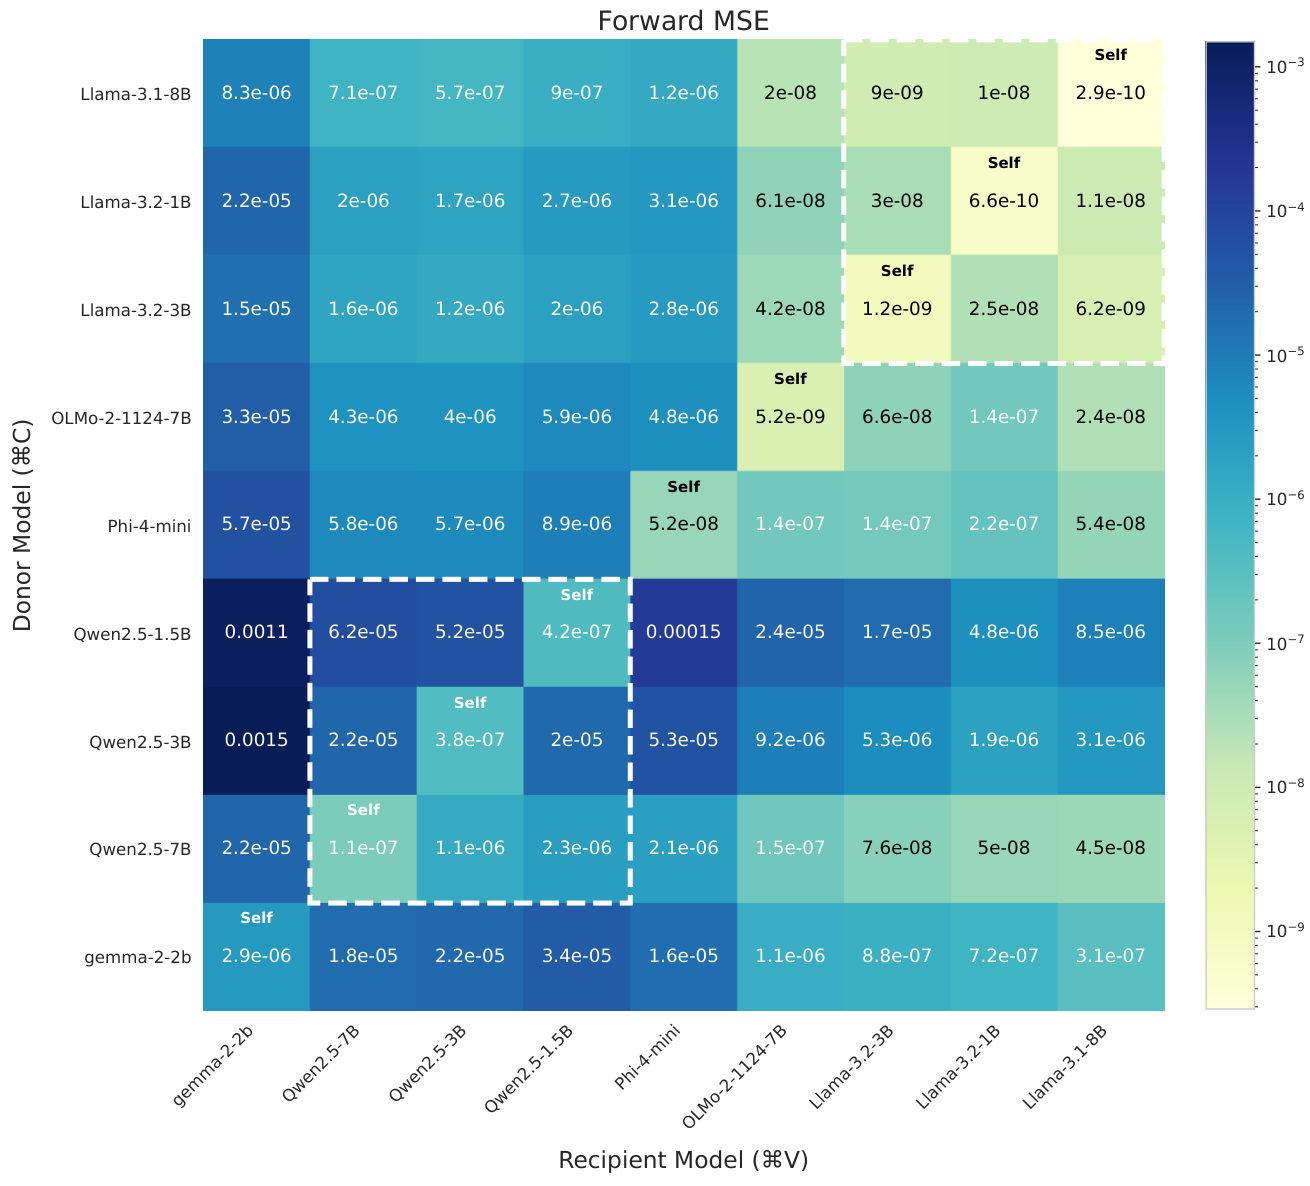
\includegraphics[width=0.8\linewidth]{figures/correlations_pseudoinverse1.png}

\vspace{0.6em}
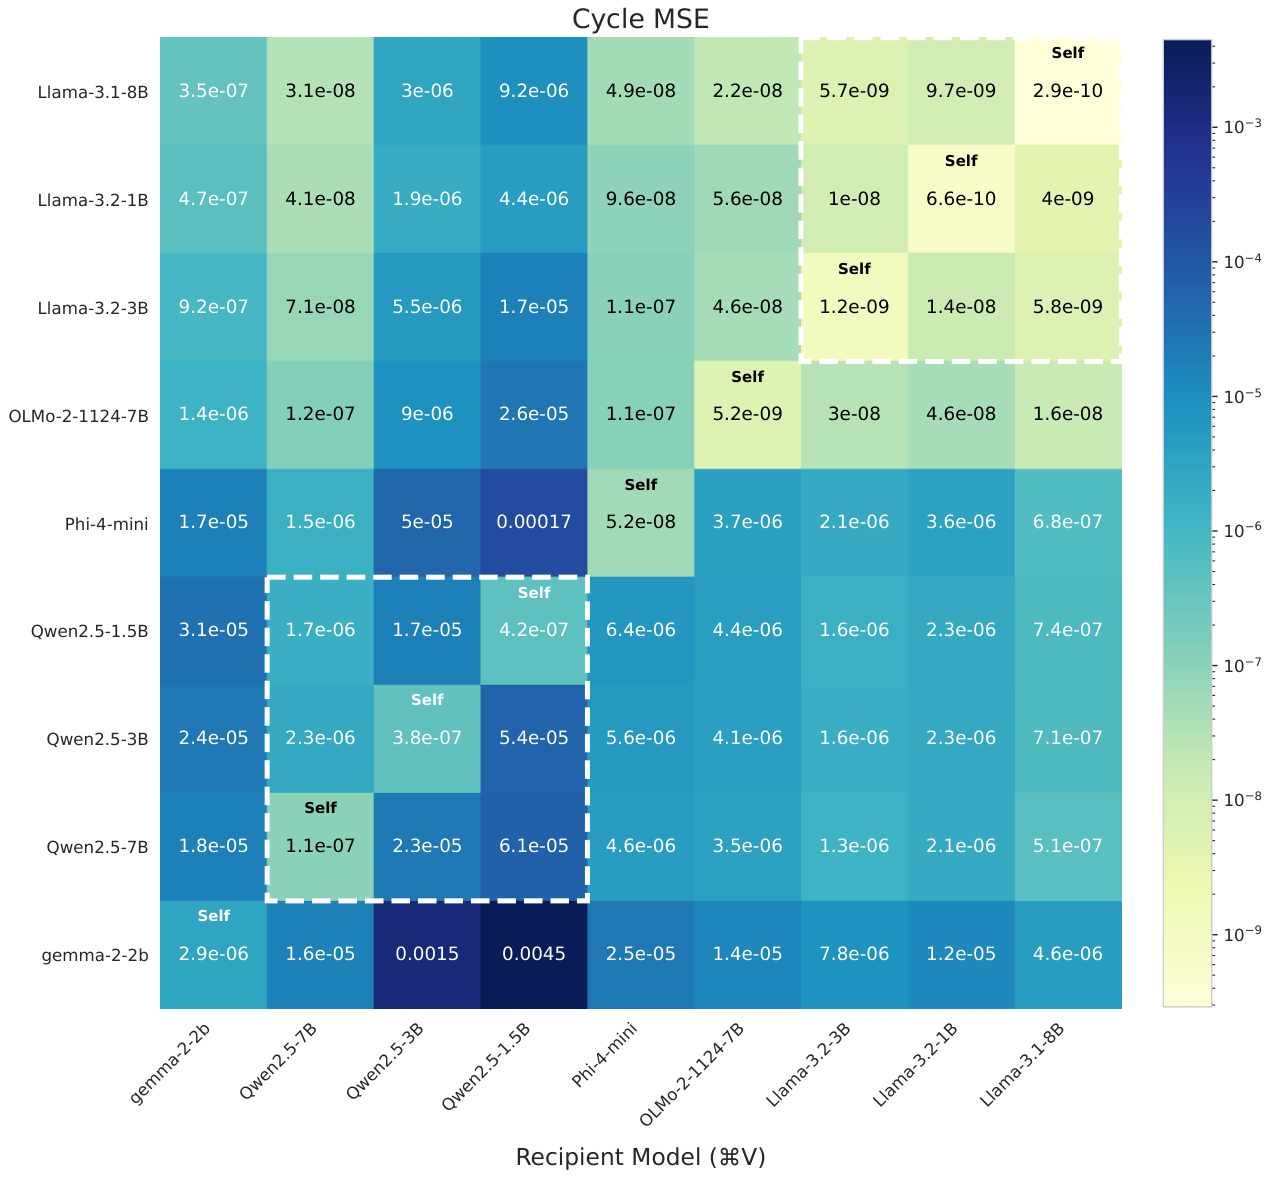
\includegraphics[width=0.8\linewidth]{figures/correlations_pseudoinverse2.png}
\caption{Forward (top) and cycle (bottom) training MSE of pseudoinverse residual-layer converters.
Same-family pairs are marked with a white square.
Values are unnormalized, so only entries in the same column (recipient) of the top plot and the same row (donor) of the bottom plot are comparable.}
\label{fig:converter-mse}
\end{figure}

\subsection{Converter wall time}

Deriving converters takes seconds on a laptop CPU once activation profiles exist (Figure~\ref{fig:converter-time}).

\begin{figure}[htbp]
\centering
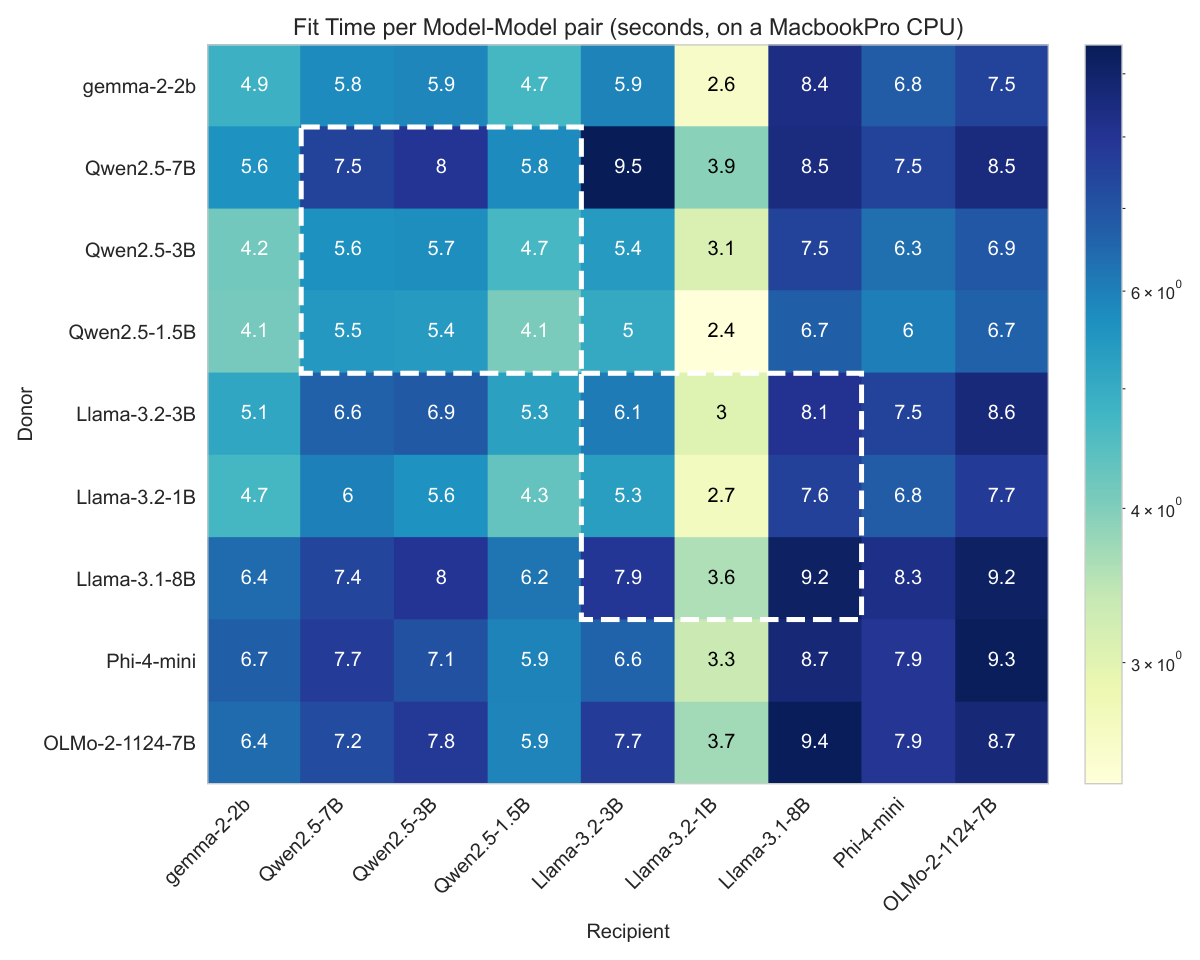
\includegraphics[width=0.8\linewidth]{figures/converter_time.png}
\caption{Pseudoinverse converter deriving time per model pair on an M1 Max CPU.}
\label{fig:converter-time}
\end{figure}
